\documentclass[a4paper, 10pt]{article}
\usepackage[margin = 1in]{geometry}
\usepackage{amsmath}
\usepackage{tabularx}
\usepackage{framed}
\setlength{\parindent}{0em}
\newcolumntype{L}{>{\arraybackslash}m{10cm}}
\newcolumntype{T}{>{\arraybackslash}m{6cm}}
\usepackage{graphicx}
\usepackage{pdfpages}

\begin{document}

\section*{Topic 12 - Superposition}

\section{Principle of superposition}
\begin{framed}
   The \textbf{Principle of superposition} states that when two or more waves of the same kind meet at a point in space, the resultant displacement at that point is equal to the vector sum of the displacements of the individual waves at that point
\end{framed}	

\section{Stationary waves}

\begin{framed}
   A \textbf{Stationary wave} is the result of interference between two progressive waves of the same type, frequency, amplitude, and speed, travelling along the same line but in opposite directions
\end{framed}	

\subsection{Properties of stationary wave}
\begin{center}
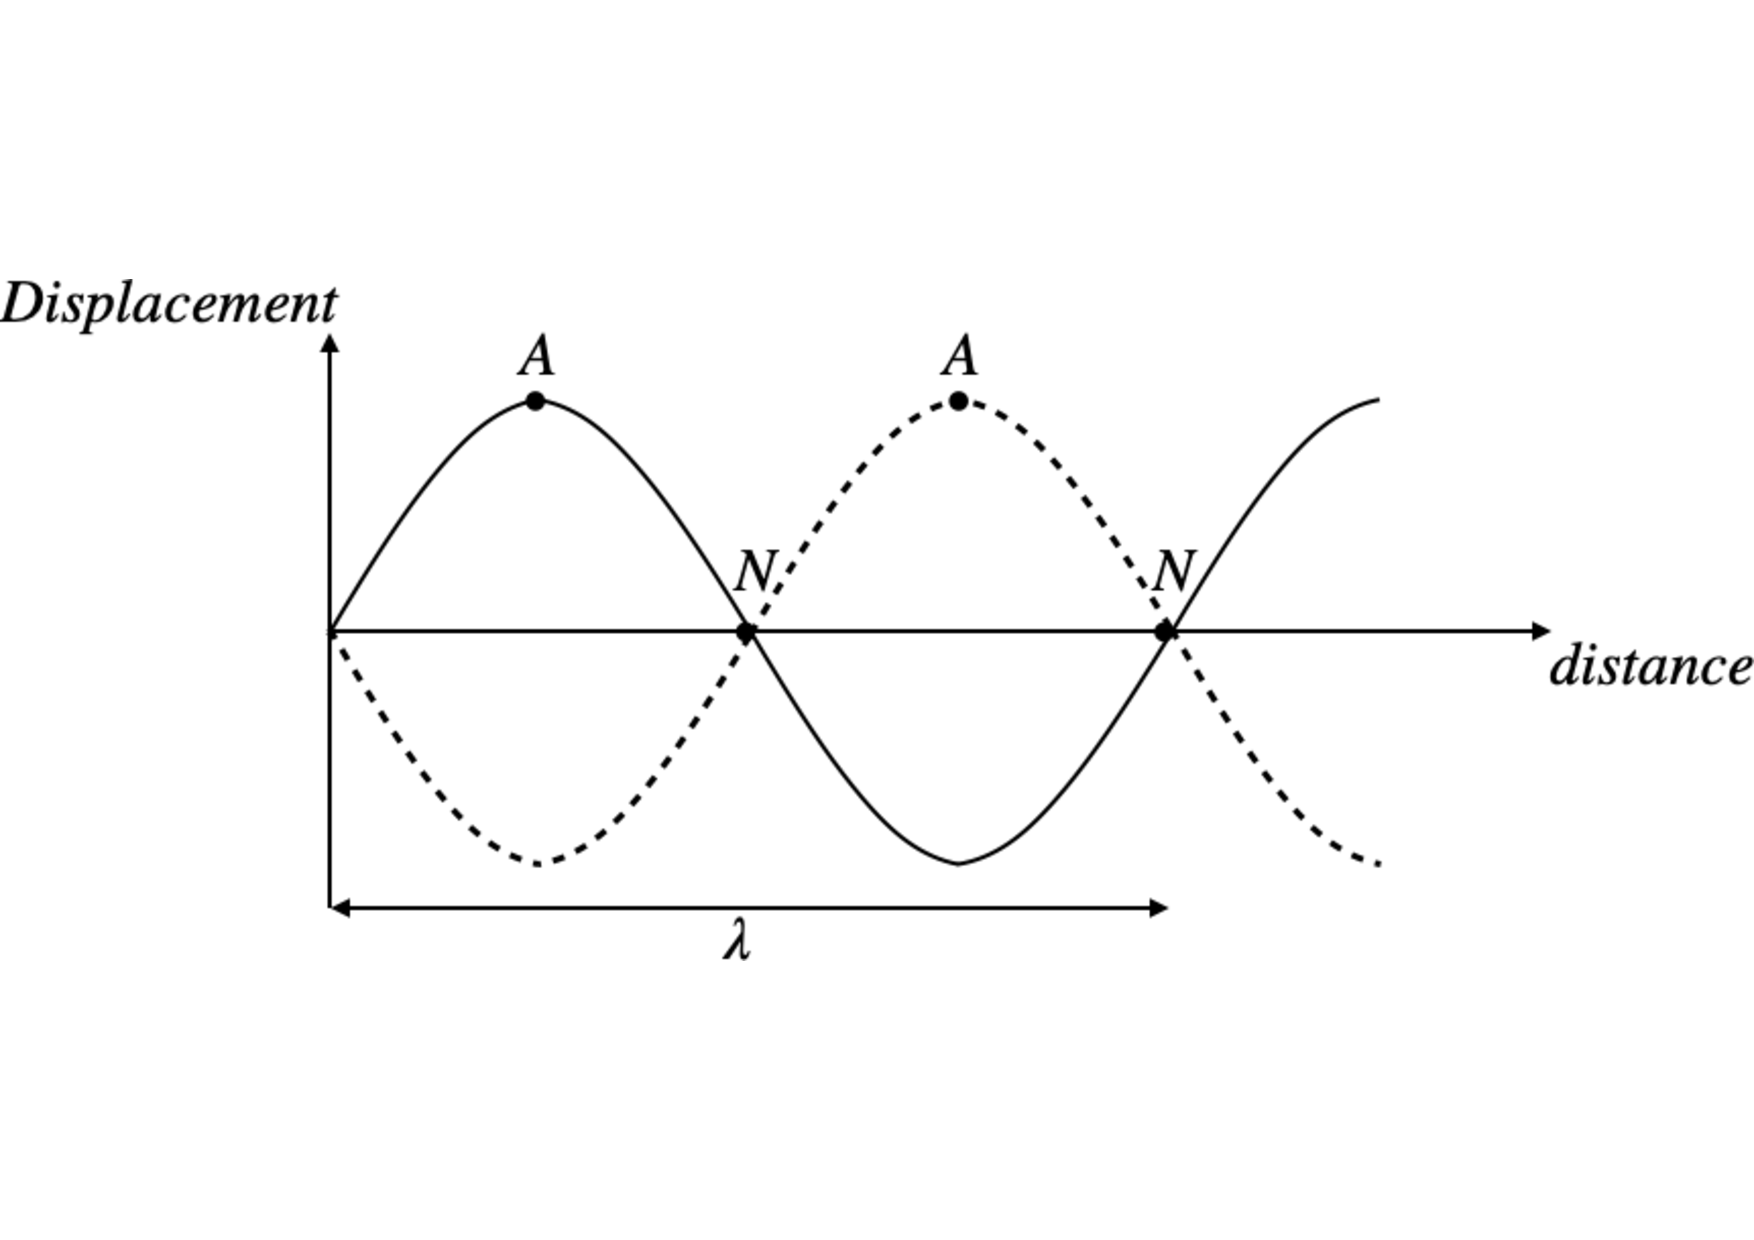
\includegraphics[trim = 50 50 50 50, width=3in]{figures/1.pdf} 
\end{center}	
\begin{itemize}
   \item The wave profile does not propagate
   \item Every particle of the wave oscillate about their respective equilibrium positions with the \textbf{same freqency} but \textbf{difference amplitude}
   \item The \textbf{antinode} is a point in a standing wave of maximum amplitude. The waves arrive \textbf{in phase}
   \item The \textbf{node} is a point of zero amplitude. The waves arrive \textbf{anti-phase} at the nodes
   \item Within two adjacent nodes, all particles oscillate \textbf{in phase} i.e. they reach their respective maxima / minima / equilibrium position at the same time
   \item particles in neighbouring segments vibrate $\pi$ out of phase with each other 
   \item distance between two adjacent nodes is \textbf{$\frac{1}{2}\lambda$}
   \item the \textbf{envelope} is a curve outlining the amplitudes of a standing wave

\end{itemize}	

\subsection{Comparing standing and progressive waves}
\begin{center}
   \begin{tabular}{c | T | T}
      Property & Progressive wave & stationary wave \\
      \hline 
      Waveform & propagates with the velocity of wave & does not propagate \\ 
      \hline
      Energy & transports energy & does not transport energy \\
      \hline
      Amplitude & all particles have the same amplitdue & Amplitude varies (from 0 to maximum) \\
      \hline
      Phase & All particles within one wave length have different phases & All particles between two adjacent nodes have the same phase. Particles in adjacent segments have $\phi = \pi$ \\
      \hline
      Freqeuncy & All points vibrate in SHM with same frequency & All points vibrate in SHM with same frequency (except at nodes) \\
      \hline
      Wavelength & equals to the distance between consecutive points in phase & equal to the distance beteen two adjacent nodes or two adjacent anti-notes \\
      \hline

   \end{tabular}
\end{center}



\subsection{Stationary waves in strings}
when a string of length $L$ that is fixed at both ends is plucked, standing waves of different frequencies are set up \\
\begin{framed}
\begin{minipage}{0.5\textwidth}
   \begin{center}
   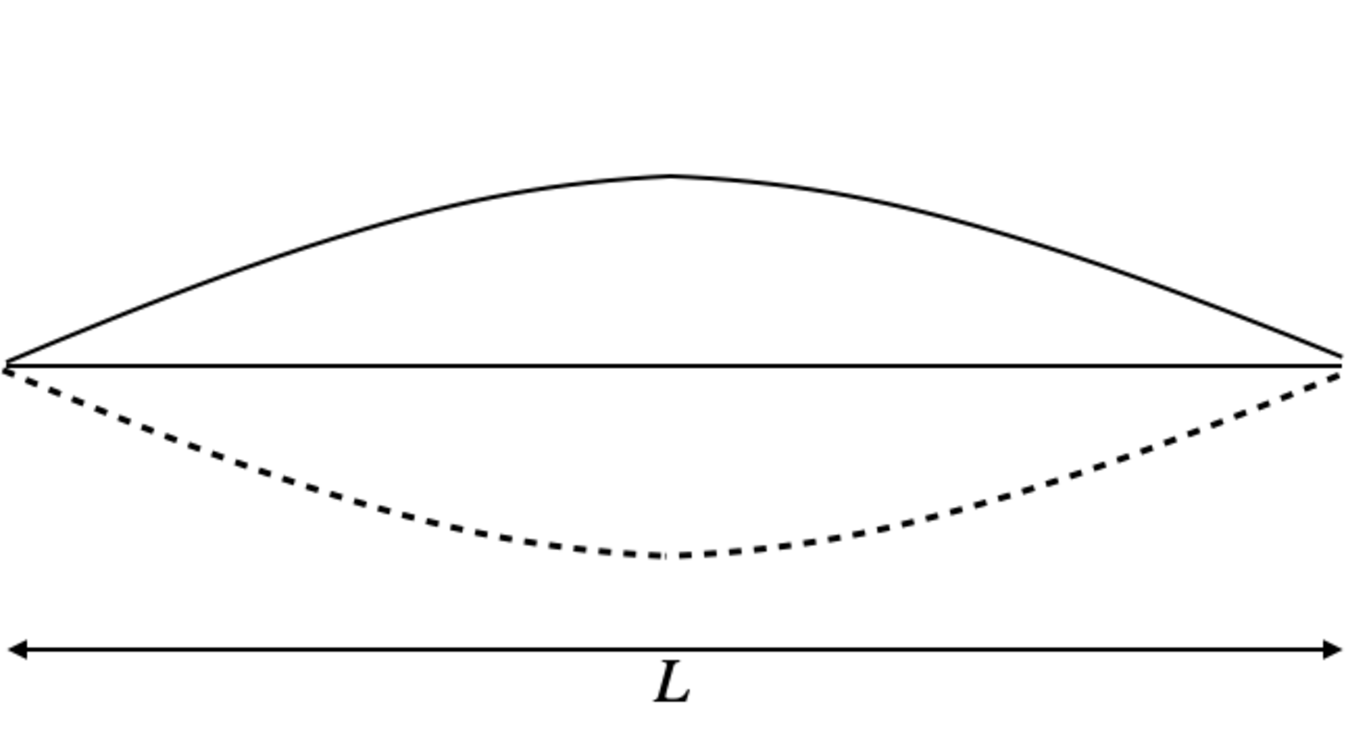
\includegraphics[trim = 50 50 50 50, width=3cm]{figures/2.pdf} 
   \end{center}	
\end{minipage}	
\begin{minipage}{0.5\textwidth}
   \begin{itemize}
      \item mode of vibration: fundamental frequency 
      \item wavelength
         \[
            L = 1 \left( \frac{\lambda_1}{2} \right) 
         \]
         \[
         \lambda_1 = 2L
         \]
      \item frequency 
         \[
         f = \frac{v}{2L}
         \]
      \item first harmonic
   \end{itemize}	
\end{minipage}	 
\end{framed}	

\begin{framed}
\begin{minipage}{0.5\textwidth}
   \begin{center}
   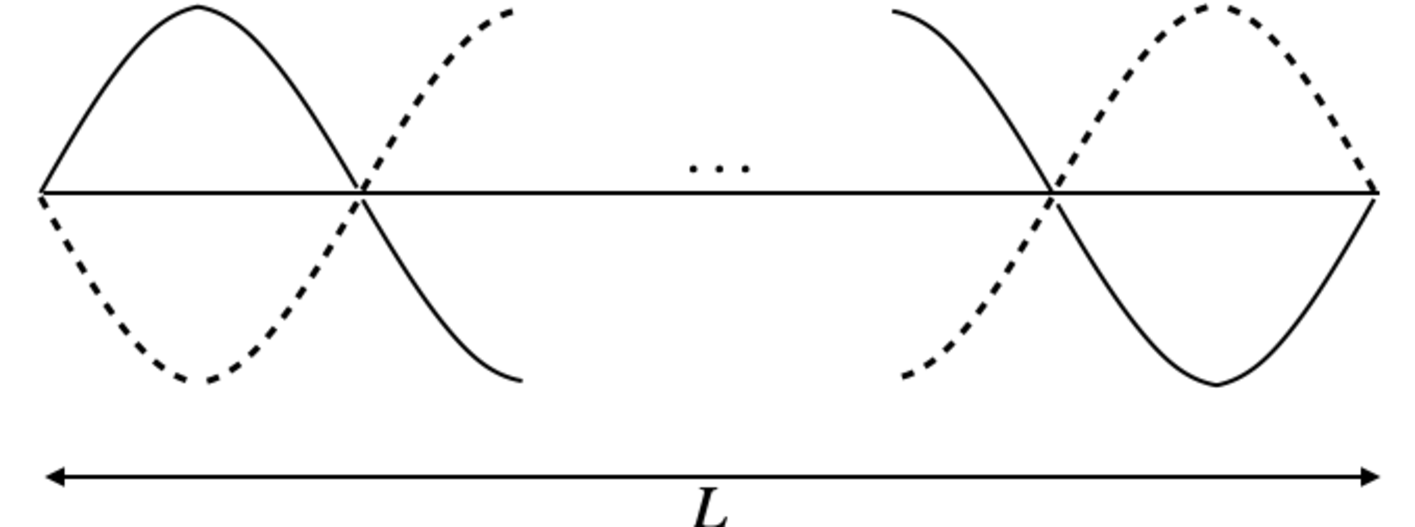
\includegraphics[trim = 50 50 50 50, width=3cm]{figures/3.pdf} 
   \end{center}	
\end{minipage}	
\begin{minipage}{0.5\textwidth}
   \begin{itemize}
      \item mode of vibration: (n-1)th overtone 
      \item wavelength
         \[
            L = n \left( \frac{\lambda_n}{2} \right) 
         \]
         \[
         \lambda_n = \frac{2L}{n}
         \]
      \item frequency 
         \[
         f = n \frac{v}{2L}
         \]
      \item $n^{th}$ harmonic
   \end{itemize}	
\end{minipage}	
\end{framed}	

\subsection{Stationary waves in air columns}
A displacement node is formed at the closed end and displacement anti-node formed at the open end
\begin{framed}
\begin{minipage}{0.5\textwidth}
   \begin{center}
   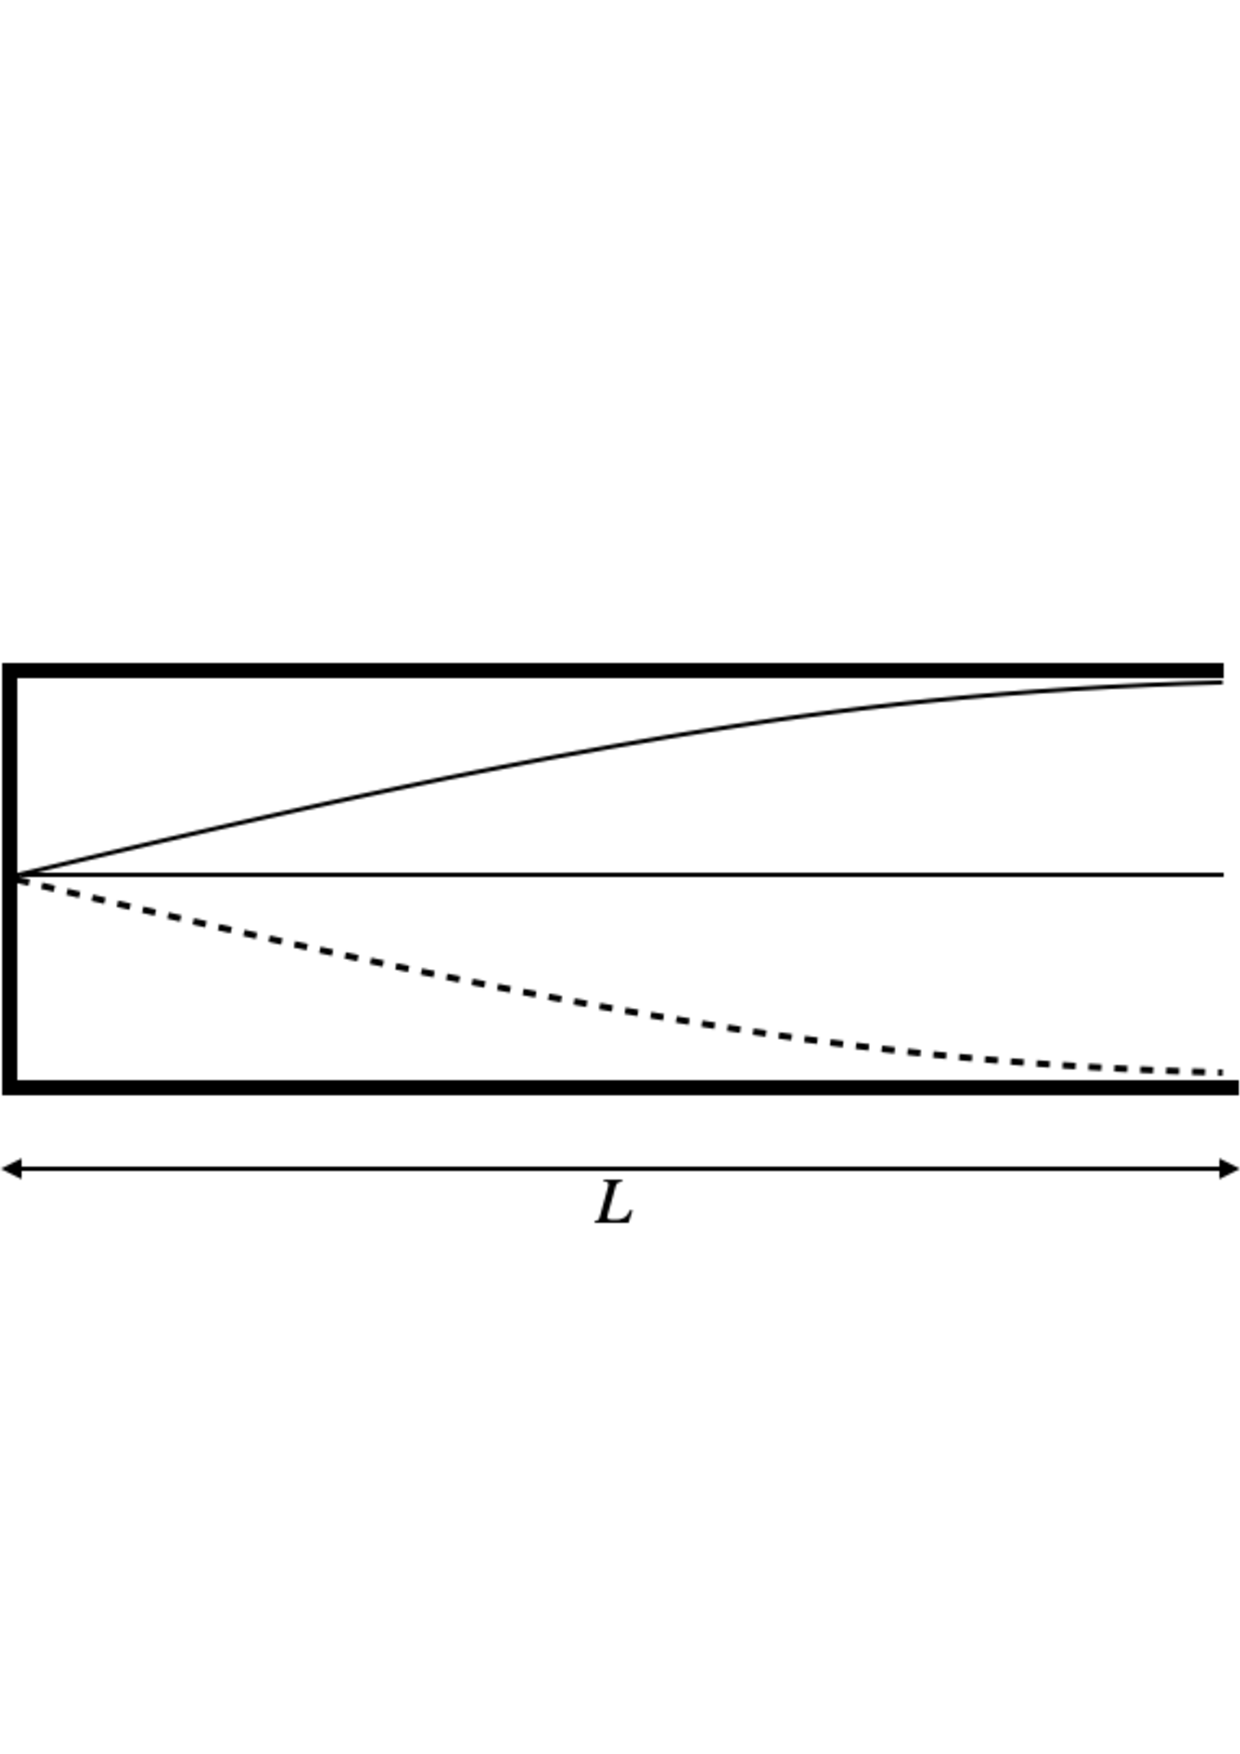
\includegraphics[trim = 50 50 50 50, width=3cm]{figures/4.pdf} 
   \end{center}	
\end{minipage}	
\begin{minipage}{0.5\textwidth}
   \begin{itemize}
      \item mode of vibration: fundamental frequency 
      \item wavelength
         \[
            L = 1 \left( \frac{\lambda_1}{4} \right) 
         \]
         \[
         \lambda_1 = 4L
         \]
      \item frequency 
         \[
         f = \frac{v}{4L}
         \]
      \item first harmonic
   \end{itemize}	
\end{minipage}	 
\end{framed}	

\begin{framed}
\begin{minipage}{0.5\textwidth}
   \begin{center}
   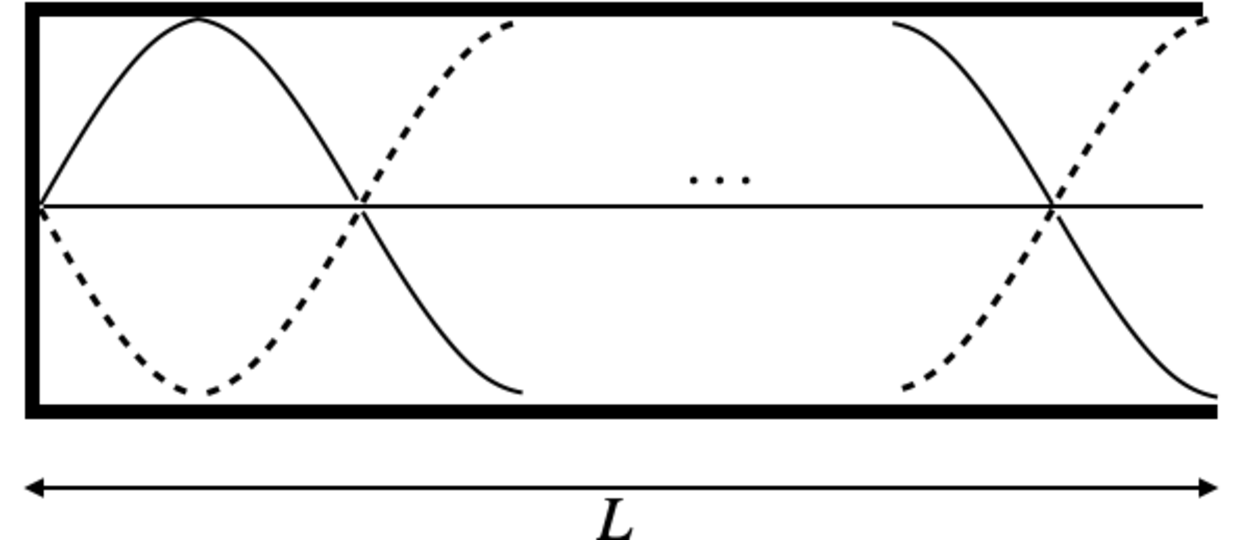
\includegraphics[trim = 50 50 50 50, width=3cm]{figures/5.pdf} 
   \end{center}	
\end{minipage}	
\begin{minipage}{0.5\textwidth}
   \begin{itemize}
      \item mode of vibration: (n-1)th overtone 
      \item wavelength
         \[
            L = (2n-1) \left( \frac{\lambda_{2n-1}}{4} \right) 
         \]
         \[
            \lambda_{2n-1} = \frac{4L}{2n-1}
         \]
      \item frequency 
         \[
            f = (2n-1) \frac{v}{4L}
         \]
      \item $(2n-1)^{th}$ harmonic
   \end{itemize}	
\end{minipage}	
\end{framed}	

\subsection{Stationary waves in pipes}
Displacement anti-node at both ends
\begin{itemize}
   \item displacement antinodes are \textbf{pressure nodes} i.e. least variation in pressure
   \item displacement nodes are \textbf{pressure anti-nodes}, largest variations in pressure
\end{itemize}	
\begin{framed}
\begin{minipage}{0.5\textwidth}
   \begin{center}
   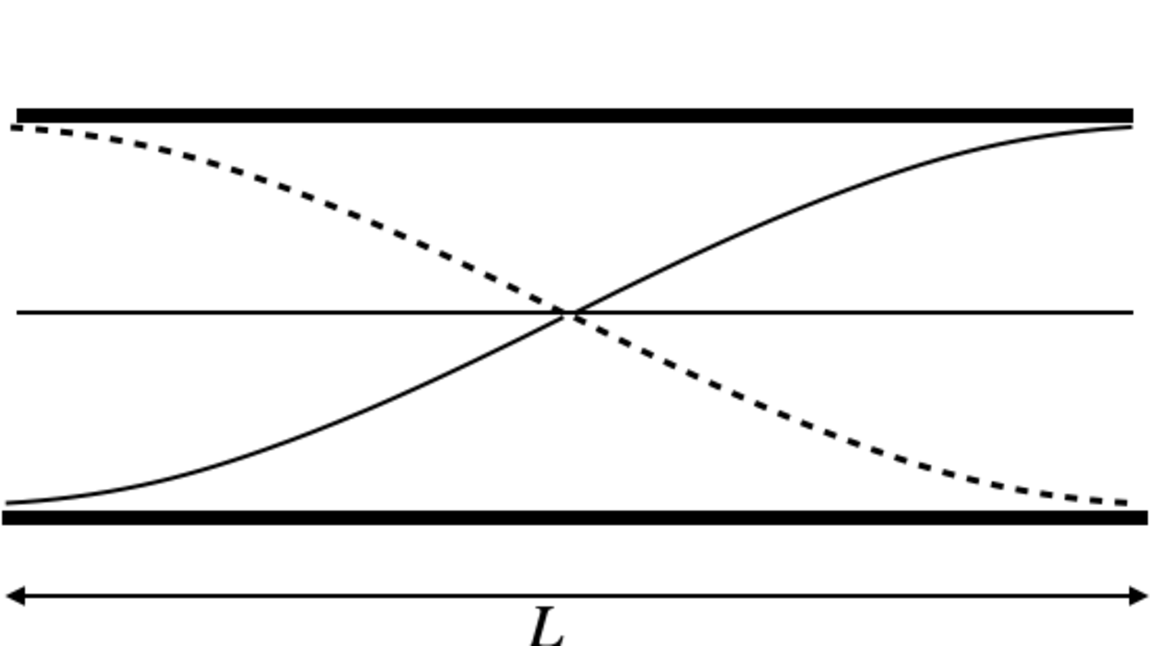
\includegraphics[trim = 50 50 50 50, width=3cm]{figures/6.pdf} 
   \end{center}	
\end{minipage}	
\begin{minipage}{0.5\textwidth}
   \begin{itemize}
      \item mode of vibration: fundamental frequency 
      \item wavelength
         \[
            L = 1 \left( \frac{\lambda_1}{2} \right) 
         \]
         \[
         \lambda_1 = 2L
         \]
      \item frequency 
         \[
         f = \frac{v}{2L}
         \]
      \item first harmonic
   \end{itemize}	
\end{minipage}	 
\end{framed}	

\begin{framed}
\begin{minipage}{0.5\textwidth}
   \begin{center}
   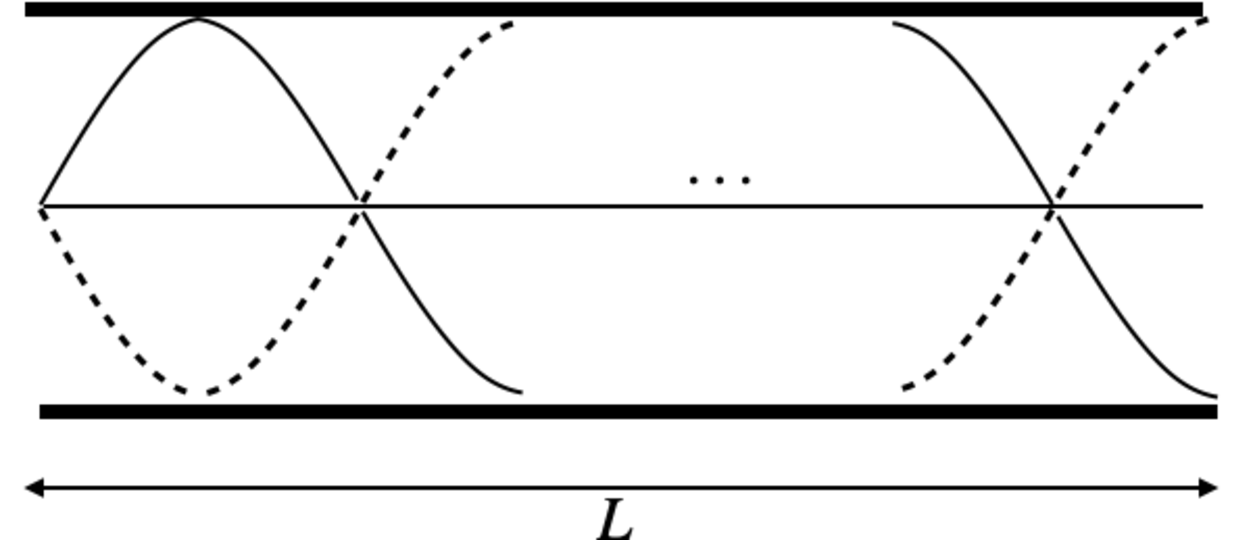
\includegraphics[trim = 50 50 50 50, width=3cm]{figures/7.pdf} 
   \end{center}	
\end{minipage}	
\begin{minipage}{0.5\textwidth}
   \begin{itemize}
      \item mode of vibration: (n-1)th overtone 
      \item wavelength
         \[
            L = 2 \left( \frac{\lambda_{n}}{2} \right) 
         \]
         \[
            \lambda_{n} = \frac{2L}{n}
         \]
      \item frequency 
         \[
         f = n \frac{v}{2L}
         \]
      \item $n^{th}$ harmonic
   \end{itemize}	
\end{minipage}	
\end{framed}	

\subsection{End correction}
the displacement antinodes at open ends of pipes are located slightly outside the pipe, hence when calculating wavelength, substitute
\[
   L = L_{actual} + c \ or\ L = L_{actual} + 2c
\]

\section{Diffraction}
\begin{framed}
   \textbf{Diffraction} is the bending or spreading of waves after passing through an aperture or round an obstacle
\end{framed}	
\begin{itemize}
   \item Diffraction is pronouned when the wavelength of thewave i of the same order of magnitude as the width of the aperture or obstacle
\end{itemize}	

\section{Coherence and Interference}
\subsection{Coherence}
\begin{framed}
   Waves or sources are \textbf{coherent} if they have a constant phase difference
\end{framed}	
\subsection{Interference}
\begin{framed}
   Interference is the \textbf{superposition} of two or more coherent waves to give a resultant wave whos resultant amplitdue is given by the principle of superposition
\end{framed}	
\begin{itemize}
   \item constructive interference: when two waves arrive with a phase difference of zero
   \item destructive interference: when two waves arrive with a phase difference of $\pi rad$
\end{itemize}	

\subsection{Two source interference}
For a two source interference to be observable
\begin{itemize}
   \item sources must be coherent
   \item waves must have similar amplitude
   \item waves must overlap and be of the same type
   \item Transverse waves must be unploarised or polarised in the same plane
\end{itemize}	

\subsection{Path difference}
\begin{framed}
   \textbf{Path difference} is the difference in distance each wave travels from its source to the point where the two waves meet
\end{framed}	

\begin{center}
   \begin{tabular}{c | c | c}
      & 2 sources in phase & 2 sources $\pi$ out of phase \\
      \hline
      Constructive interference & $\Delta L = n \lambda$ & $\Delta L = (n + \frac{1}{2}) \lambda$  \\
      \hline
      Destructive interference & $\Delta L = (n+ \frac{1}{2}) \lambda$ & $\Delta L = n \lambda$  \\
      \hline
   \end{tabular}
\end{center}

\section{Double slit experiment}
\begin{minipage}{\textwidth}
   \begin{center}
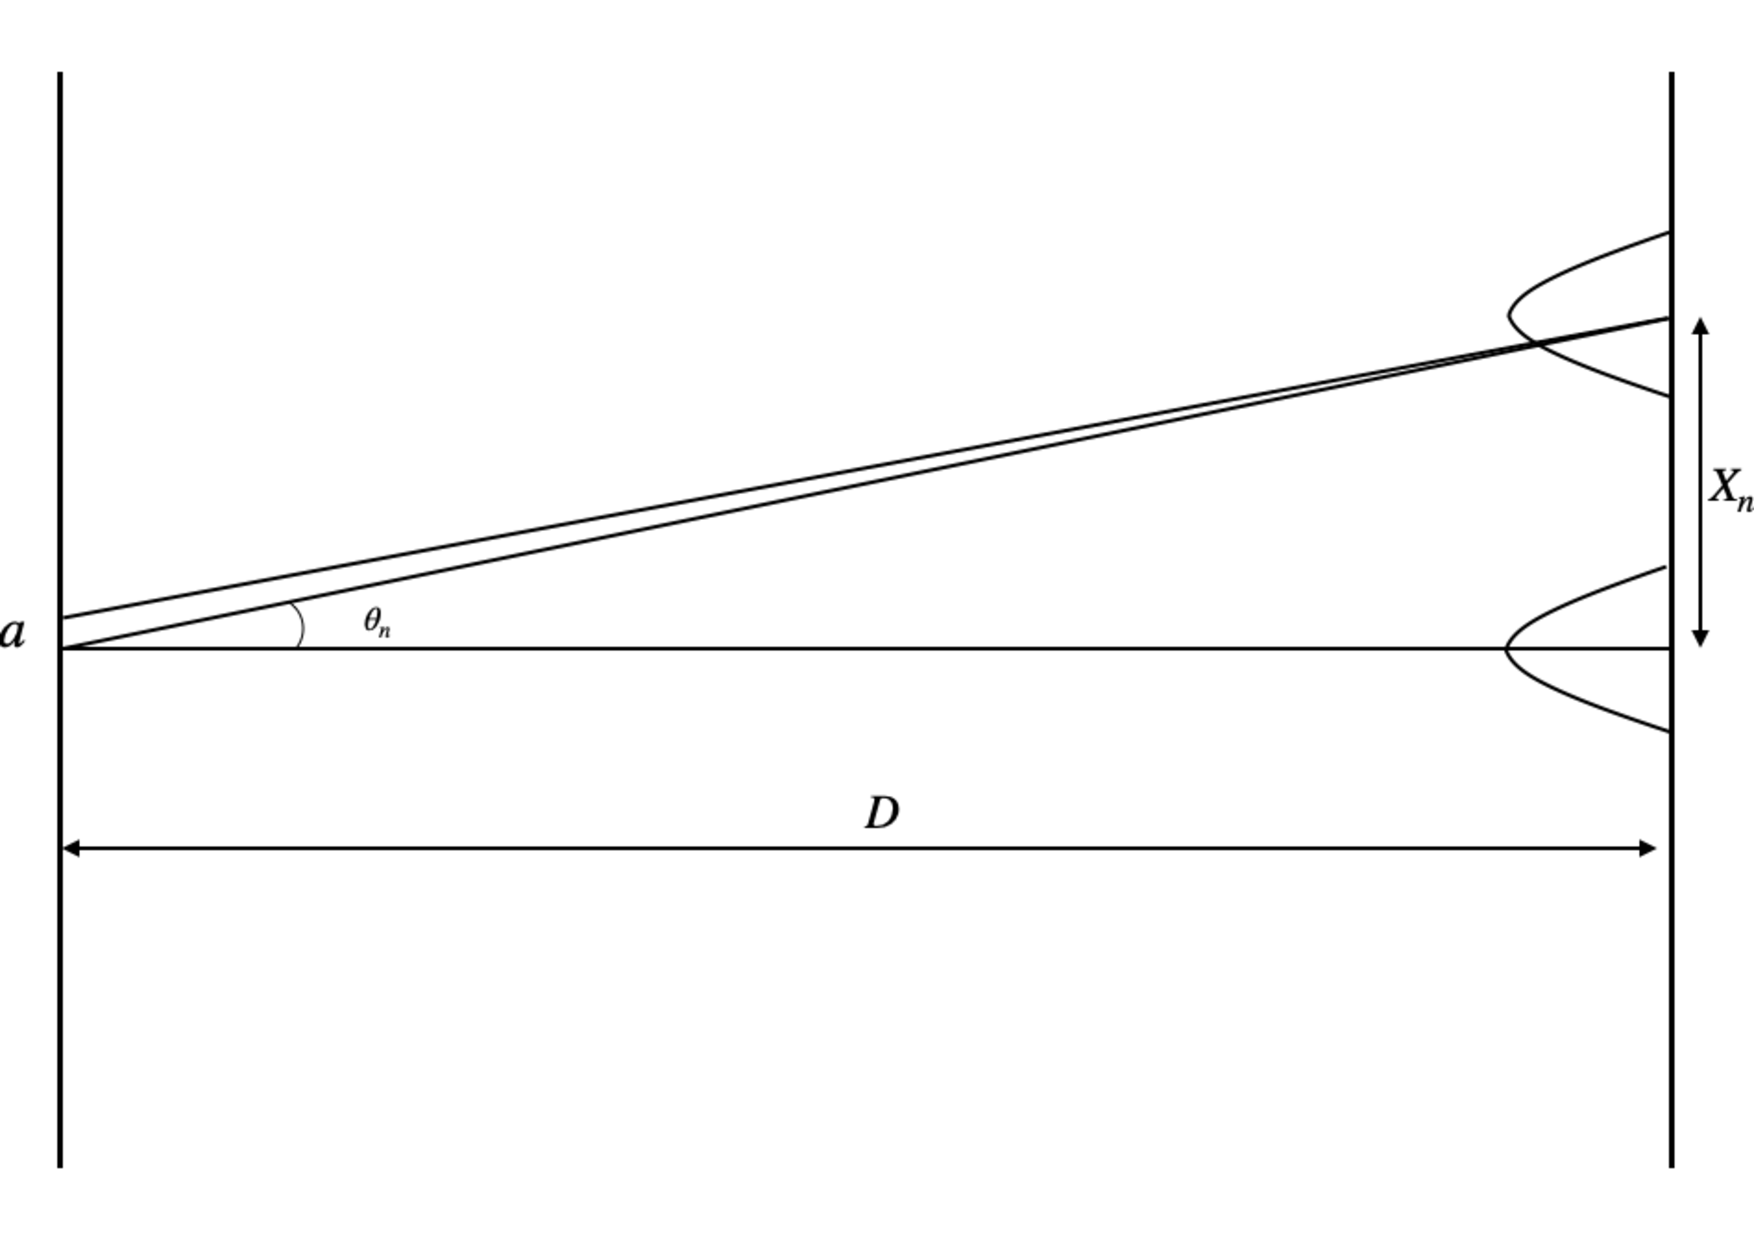
\includegraphics[trim = 50 50 50 50, width=3in]{figures/8.pdf} 
   \end{center}	
\end{minipage}	

Assuming $a << D$, and hence light rays almost parallel, then 
\[
   \text{path difference} = \Delta x = asin \theta_n
\]

For constructive interference at the $n^{th}$ bright fringe
\[
a sin \theta_n = n \lambda
\]
\[
sin \theta_n = \frac{n\lambda}{a}
\]

Additionally,
\[
tan \theta_n = \frac{X_n}{D}
\]

Assuming \textbf{$a >> lambda$}, $\theta$ is small 
\[
   sin \theta_n \cong tan \theta_nn
\]
\[
\frac{n\lambda}{a} \cong \frac{X_n}{D}
\]

Hence constructive intereference takes place at 
\[
X_n = \frac{n \lambda D}{a}
\]

Fringe separation is thus
\[
   x = X_n - X_{n-1} = \frac{\lambda D}{a}
\]


\section{Diffraction grating}
For a diffraction grating of $N$ lines per meter, slit separation is 
\[
d = \frac{1}{N}
\]
Path difference is 
\[
\Delta x = d sin \theta_n
\]

Assuming $d << D$, constructive interference occur 
\[
d sin \theta_n = n\lambda
\]
since $\theta_n < 90^{\circ}$ 
\[
sin \theta_n < 1
\]
\[
\frac{n\lambda}{d} < 1
\]
\[
n < \frac{d}{\lambda}
\]



\section{Single slit interference}
\begin{framed}
   \textbf{Huygens' Principle} states that at any instant, all points on a wavefront could be recarded as secondary sources giving rise to their own outward spreading circular wavelets. \\

   the envelope of wavefronts produced by each secondary source gives the new position of the wavefront
\end{framed}	

For a single slit diffraction with slit separation $b$ , for $b << D$, position of the first minima is given by
\[
bsin \theta = \lambda
\]
\[
sin \theta = \frac{\lambda}{b}
\]

using arc length where \[
   s = r \theta
\]
for small $\theta$ the width, $y$  of the central bright fringe is 
\[
   y = D(2 \theta) = \frac{2D\lambda}{b}
\]


\section{Rayleigh criterion}
\begin{framed}
   The \textbf{resolving power} of a single slit is the ability to distinguish between closely spaced objects
\end{framed}	
\begin{framed}
   \textbf{Rayleigh's criterion} states that two objects are just resolved when the central maximum of one iamge falls on the first minimum of thee other image. The criterion is satisfied when the mimimum angular separation of the sources $\theta_{min}$ is
   \[
      \theta_{min} = \frac{\lambda}{b}
   \]
   
\end{framed}	











\end{document}	
